\documentclass[11pt,a4paper]{article}

\usepackage[margin=1in]{geometry}
\usepackage{amsmath}
\usepackage{amssymb}
\usepackage{amsthm}
\usepackage{array}
\usepackage{booktabs}
\usepackage{placeins}
\usepackage{needspace}
\usepackage{listings}
\usepackage{pgfplots}
\pgfplotsset{compat=1.17}
\usetikzlibrary{decorations.pathreplacing}
\widowpenalty=10000
\clubpenalty=10000

% Two stacked figures may share a page with running text beneath them, a tall float may take most of a
% page that still carries prose, and a float page must be nearly full before one is made: the barriers
% that keep tables out of mid-sentence would otherwise strand half-empty pages at every flush.
\setcounter{topnumber}{2}
\setcounter{bottomnumber}{2}
\renewcommand{\topfraction}{0.9}
\renewcommand{\bottomfraction}{0.7}
\renewcommand{\textfraction}{0.07}
\renewcommand{\floatpagefraction}{0.85}
\lstdefinestyle{walk}{basicstyle=\small\ttfamily, mathescape=true, columns=fullflexible,
  keepspaces=true, frame=single, framesep=6pt, xleftmargin=2pt, xrightmargin=2pt}
\usepackage[numbers]{natbib}
\usepackage[hidelinks,unicode]{hyperref}

\newcommand{\doi}[1]{\href{https://doi.org/#1}{\nolinkurl{doi:#1}}}

% Modest stretch tolerance for the inline code vocabulary; without it single lines overfill by about a point.
\emergencystretch=1em

\hypersetup{
  pdftitle={Certified Panic Mode: Repair-Invariant Error Recovery for Maximal-Munch Lexing},
  pdfauthor={Nicklas Nidhögg},
  pdfsubject={Lexical error recovery; deterministic finite automata; maximal munch tokenization},
  pdfkeywords={error recovery, panic mode, tokenization, deterministic finite automata, maximal munch}
}

\theoremstyle{definition}
\newtheorem{definition}{Definition}

\theoremstyle{plain}
\newtheorem{lemma}{Lemma}
\newtheorem{theorem}{Theorem}
\newtheorem{corollary}{Corollary}
\newtheorem{proposition}{Proposition}
\newtheorem{assumption}{Assumption}

\theoremstyle{remark}
\newtheorem{remark}{Remark}

\newcommand{\code}[1]{\texttt{#1}}
\newcommand{\Rreach}{R_{\mathrm{reach}}}
\newcommand{\Rcomp}{R_{\mathrm{complete}}}
\newcommand{\suffix}[2]{#1[#2..]}
\newcommand{\prefix}[2]{#1[0..#2)}
\newcommand{\window}[3]{#1[#2..#3)}
\newcommand{\con}{\operatorname{con}}

% Float pages stack their floats at the top with a small fixed gap, the slack all at the bottom, instead of
% stretching a third of a page of glue between two tables.
\makeatletter
\setlength{\@fptop}{0pt}
\setlength{\@fpsep}{18pt plus 6pt}
\setlength{\@fpbot}{0pt plus 1fil}
\makeatother

\title{Certified Panic Mode:\\Repair-Invariant Error Recovery for Maximal-Munch Lexing}
\author{Nicklas Nidh\"ogg\\[0.4em] \normalsize Independent Researcher\\ \normalsize
\texttt{nicklas.nidhogg@gmail.com}\\ \normalsize ORCID: 0009-0006-6161-6150}
\date{September 6, 2026}

\begin{document}

\maketitle

\begin{abstract}
Classical panic-mode recovery skips a failed scan forward by convention: it promises progress, and
membership in a designated set where one is found, but no repair-universal boundary guarantee for the
position it lands on. This paper chooses the resume position by theorem: a position is a sound recovery point when
every prefix repair whose scan commits through the certificate's returned evidence places a token boundary
there, complete repairs the special case, by a committed-prefix lemma over certificates posted for a
different purpose (arXiv:2608.03473, arXiv:2608.09761). The quantifier is strictly the stronger one, and a
dichotomy locates the difference exactly: the inclusion is strict precisely when no repair completes
while some scan still commits through the evidence, a two-token witness realizing the case. The evidence-returning form
pairs each answer with the interval it rests on, which is what makes the guarantee deployable: a caller
who knows what the scanner cannot check decides whether the certified boundary transfers to the clean
input it intended. The search is one forward walk in evidence order and provably terminates; the
guarantee is per-automaton, relative to the active mode. The procedure ships in the munch lexing
library, and a deterministic corruption study measures its recovery quality beside the classical skip-one
and delimiter conventions. Every certified answer whose evidence survives the damage passes its executable
landing check on every recovery move, $40{,}885$ of $40{,}885$; among first answers, the $5{,}595$ resting
on evidence the damage reached land $1{,}589$ times, reported and never asserted. On $13{,}522$ of the
$16{,}808$ trials the shipped repair routine labels beyond repair, the resumed suffix tokenizes whole and
the two quantifiers provably coincide, so both are empty there if those negative labels are exact;
$3{,}286$ stay undetermined.
\end{abstract}

\section{Introduction}

Two companion papers certify positions in completely tokenizable input: a certified split byte begins a token at
every occurrence in every completely tokenizable input, and a certified split window places a token origin at a
fixed offset into every occurrence~\citep{splitpoints2026, splitwindows2026}. Error recovery lives exactly where
those hypotheses fail, in input that is not completely tokenizable. The classical answer is panic mode, at two
levels: the lexical form deletes characters until a well-formed token appears, and the parser form discards to a
designated synchronizing delimiter, a newline or a semicolon. Both are old and widespread; both promise progress
and, where a synchronizer is found, membership in the designated set, and neither supplies a repair-universal
boundary guarantee for the position landed on; and this study transplants the delimiter convention down a level
to evaluate it, in both placements, beside the lexical form. This paper supplies the theorem the convention
never had: the same static certificates that plan parallel chunk boundaries in valid input certify
resynchronization points in broken input, with a guarantee quantified over every prefix repair whose scan
commits through the certificate's preserved evidence.

Three naive statements fail, and their failures shape the definition. First, demanding that the resumed suffix
tokenize on its own is insufficient rather than wrong: over $\{\code{ab}, \code{b}\}$ the suffix \code{b}
tokenizes alone, yet the repair \code{a} produces the whole \code{ab}, one token with no boundary at the cut, so
standalone suffix tokenizability filters positions without aligning any of them with a repaired whole. Second, a
certified window with positive origin spans bytes before the position it certifies, so the resumed suffix alone
does not contain the occurrence the certificate speaks about; a statement quantifying only over the suffix
cannot use the window theorem. Third, the prefix guarantee of the split-points paper speaks about the tokens
committed before a failure, never about how to continue past it. The definition that survives all three is
repair invariance: a position is a sound recovery point when every repair of the broken prefix whose scan
commits through the certificate's evidence places a committed token boundary there, complete tokenizability the
corollary case. It quantifies over repaired inputs rather than bare suffixes, which defeats the first failure;
the theorems' anchor conditions pin the certificate's evidence inside the unmodified region, which defeats the
second; and it is a statement about continuation past the failure, not about the tokens committed before it,
which is what the third failure asks for.

The results are one-line consequences of the posted certificates, and that is the point: nothing new needs to be
proved about the automaton, only the right question asked of theorems that already exist. The contribution is
the recovery contract and its operational validation, not a third certificate construction. Certified bytes are
repair-invariant at their own position; certified windows at their occurrence plus the certified origin, under
the one extra constraint that the repair leave the occurrence intact, which the searching algorithm satisfies by
construction because it only reports evidence lying wholly at or after its own search anchor. Whether the text
past that anchor is truly unmodified is the caller's trust decision, and the evaluation prices it. A progress
lemma makes the scan-and-recover loop terminate, and mode-driven scanning gets a per-automaton certificate,
relative to the active mode, never a theorem over repairs that change modes. The procedure ships in the munch
lexing library~\citep{munch}, and the evaluation measures what the theorem is worth against the conventions it
replaces: quality, not throughput.

The contributions:
\begin{itemize}
\item Repair-invariant resynchronization, a definition of recovery-point soundness that quantifies over
every prefix repair whose scan commits through the certificate's evidence, complete repairs the special case, with
the three naive alternatives shown to fail
(Section~\ref{sec:repair}).
\item Two theorems, one per certificate kind, each a short consequence of the companions' posted
results, plus the progress lemma and the mode-scope remark that state a driver's obligations
(Section~\ref{sec:repair}).
\item The searching primitive and its driver as shipped, with the one deliberate divergence from the
planners' certificate policy explained, and the fail-closed fixtures that pin each layer
(Sections~\ref{sec:search} and~\ref{sec:impl}).
\item A deterministic corruption study whose oracle is exact for the theorem-predicted boundary
consequence on the exhibited pristine repair: the pristine corpus itself supplies the repair the
theorems quantify over, so the landing check runs on every returned answer whose supporting evidence the
damage spares,
rather than on a sample; the library's anchored complete-repair decider is evaluated beside the walk under
its documented contract, blind and oracle-anchored, a different-property comparator with repairability
stratifying every trial; classical skip-one and skip-to-delimiter
conventions are measured beside it (Section~\ref{sec:eval}).
\end{itemize}

The logical chain, in one paragraph. The paper separates three questions a damaged scan raises: whether
any repair completes the input, whether a returned position is a boundary under every repair whose scan
commits through its evidence, and how often, under measured damage, that evidence survives. Certificates from the
companion papers identify positions; the resynchronization theorems transfer their guarantee to every
evidence-reaching repair of a failed scan's prefix; the collapse proposition and its dichotomy corollary
locate exactly where the strengthened quantifier adds content; the overhang lemma tells a caller when
coverage is forced by arithmetic alone; and the campaign measures availability, coverage, and displacement
where the theorems' premises hold and where they fail.

\section{Preliminaries}

The model is the companions', restated and not reproved. A token set compiles to a deterministic finite
automaton scanned by the usual longest-match loop: from an offset the scanner consumes bytes while transitions
are defined, remembers the last accepting position, emits the token found there, and restarts at that position
in the initial state. Emitted tokens have positive length: the committed position strictly advances, an
accepting initial state (a nullable pattern's minimization) never emits at zero width, and a scan that cannot
advance fails. Write $\mathrm{con}(x)$ for the scanner's final committed offset on input $x$; call $x$
completely tokenizable when $\mathrm{con}(x) = |x|$; and call the \emph{failure offset} of a failed scan $f =
\mathrm{con}(x)$, the final committed offset: the start of the token attempt that failed, not the read head
where the transition died, which lies at or past $f$ (equal exactly when the very first byte of the attempt has
no transition). For a scan resumed at offset $s$, the failure offset is the absolute $f_s = s +
\mathrm{con}(x[s..])$, the driver's current committed offset. The shipped driver always searches from one past
the failure offset; naming another anchor is the evaluation's oracle-aided arm and the shipped clean-anchored
interface, calling the primitive directly, never the failure-anchored driver. A byte is \emph{formally
certified} when the split-points paper's static condition holds of it, and that paper's characterization theorem
makes the condition exact: a byte is certified if and only if every occurrence of it, in every completely
tokenizable input, begins a token; the characterization carries that paper's standing assumption that the
initial state is itself live. The condition is vacuously true of a byte no completely tokenizable input contains
at all, and the library reports only the \emph{useful} certified bytes, those with a live initial-state
transition, the companion's own reported class. Throughout this paper \emph{certified byte} means the reported,
useful kind: the walk, the worked example, the refusal claims, and the evaluation all speak of what the search
reports, and the vacuous case is named where it matters. A \emph{certified window} $(W, o)$ is a nonempty byte
string with a certified origin $o$, $0 \le o < |W|$: in every completely tokenizable input containing an
occurrence of $W$, the token covering the occurrence's final byte begins exactly $o$ bytes into the occurrence.
The certificate is defined for every window length; the shipped recovery walk searches lengths two to four, a
cap whose consequences Section~\ref{sec:search} owns. The window results inherit the windows paper's scope, flat
token sets with non-nullable patterns; the byte results carry no such restriction. Everything in this paper is
relative to one fixed automaton; mode-driven scanning returns in Section~\ref{sec:repair}. Both certificates are
static, computed from the automaton alone before any input exists, which is what lets a recovery built on them
promise anything about inputs it has never scanned.

\section{Repair-invariant resynchronization}
\label{sec:repair}

Let $\Sigma$ be the byte alphabet throughout.
\begin{definition}[Local repair]
For input $x$ and anchor $c$ with $0 \le c \le |x|$, a \emph{repair before $c$} is any string $r \in
\Sigma^{*}$, giving the repaired input $y = r \cdot \suffix{x}{c}$. A repair is \emph{tokenizable} when $y$ is
completely tokenizable.
\end{definition}

Nothing at or after the anchor changes; everything before it may, by outright replacement rather than only
insertion or deletion, so the results below quantify over every prefix-local fix at once.

Complete tokenizability to the end of input is the natural quantification for a whole file in hand, but it is
stronger than the certificates need, and the stronger form buys vacuity: a tail whose far end no repair can save
would escape every claim below even where the near end is perfectly ordinary. The scan itself supplies the
weaker, sharper currency. For any input $w$, write $\con(w)$ for the scan's \emph{committed length}: the sum of
the emitted token lengths when maximal munch halts, equal to $|w|$ exactly when $w$ is completely tokenizable.

\begin{lemma}[Committed prefix]
\label{lem:committed}
For any input $w$, the committed prefix $z = \prefix{w}{\con(w)}$ is completely tokenizable, and its scan emits
exactly the tokens the scan of $w$ commits.
\end{lemma}

\begin{proof}
By induction over the committed tokens. Each commit is the last accepting position on the viable run from its
token's start, and the scan of $w$ read past it only through nonaccepting states before rolling back, so
truncating $w$ at the final commit removes no accepting candidate: at every committed start, the scan of $z$
sees the same last accept and commits the same token, and the final commit lands exactly at $z$'s end.
\end{proof}

The lemma is the bridge the certificates cross: whatever a scan commits is itself a completely tokenizable
input with the identical segmentation, so any theorem quantifying over completely tokenizable inputs applies to
the committed prefix of every scan, finished or failed.

\begin{definition}[Evidence-reaching repair]
\label{def:reaching}
For evidence occupying $\window{x}{q}{q+w}$ with $c \le q$, $0 < w$, and $q + w \le |x|$, a repair $r$
before $c$ is \emph{evidence-reaching} when the scan of $y = r \cdot \suffix{x}{c}$ commits through the
evidence's image: $\con(y) \ge |r| + (q + w - c)$.
\end{definition}

Every tokenizable repair is evidence-reaching for every choice of evidence, since $\con(y) = |y|$; the reverse
fails, and that gap is the point. A repair whose scan dies far past the evidence still counts, so the
quantification below binds real, failing inputs, not only the ideal ones that tokenize to the end.

\begin{definition}[Repair-invariant resynchronization point]
Position $p$ with $c \le p < |x|$ is a \emph{repair-invariant resynchronization point} for $x$ anchored at $c$,
relative to evidence occupying $\window{x}{q}{q+w}$, if in every evidence-reaching repair $y = r \cdot
\suffix{x}{c}$, a token of the scan's committed segmentation begins at $|r| + (p - c)$.
\end{definition}

\begin{theorem}[Certified bytes resynchronize]
If $x[p]$ is a certified split byte and $c \le p$, then $p$ is a repair-invariant resynchronization point for
$x$ anchored at $c$, relative to the evidence $\window{x}{p}{p+1}$: in every repair whose scan commits through
the byte's image, a committed token begins at $|r| + (p - c)$.
\end{theorem}

\begin{proof}
Every repair anchored at or before $p$ preserves the occurrence of the certified byte at $p$'s image. When the
scan of $y$ commits through that image, the committed prefix $z$ contains it, $z$ is completely tokenizable
with the scan's own segmentation by Lemma~\ref{lem:committed}, and the byte certificate places a token origin
at every occurrence in every completely tokenizable input, the characterization theorem of the split-points
paper~\citep[Theorem~2, arXiv v2]{splitpoints2026}, so a token of $z$'s segmentation, which is the committed
segmentation of $y$, begins at the image.
\end{proof}

\begin{theorem}[Certified windows resynchronize at their origin]
For a flat token set with non-nullable patterns, the windows paper's standing scope: if $x$ carries an
occurrence of a certified window $(W, o)$ at position $q$, then $p = q + o$ is a repair-invariant
resynchronization point for $x$ anchored at any $c \le q$, relative to the evidence $\window{x}{q}{q+|W|}$:
in every repair whose scan commits through the occurrence's image, a committed token begins at $|r| + (p - c)$.
\end{theorem}

\begin{proof}
Every repair anchored at or before $q$ preserves the occurrence whole at $q$'s image. When the scan of $y$
commits through the occurrence's image, the committed prefix $z$ contains it whole and is completely
tokenizable with the scan's own segmentation by Lemma~\ref{lem:committed}, and the window certificate places
the origin of the token covering the occurrence's final byte at its image plus $o$ in every completely
tokenizable input carrying the occurrence, the certified-window contract and its soundness
theorem~\citep[Definition~1 and Theorem~1, arXiv v1]{splitwindows2026}.
\end{proof}

\begin{corollary}[Complete repairs]
\label{cor:complete}
In every tokenizable repair $y = r \cdot \suffix{x}{c}$, a token of $y$'s segmentation begins at $|r| + (p -
c)$, for $p$ and $c$ as in either theorem.
\end{corollary}

\begin{proof}
A tokenizable repair commits its whole input, $\con(y) = |y|$, so it is evidence-reaching for any evidence,
and its committed segmentation is its segmentation.
\end{proof}

The corollary is the quantification an earlier version of this paper proved directly, and it is the weaker
claim. For an anchor $c$ and evidence $\window{x}{q}{q+w}$, write
\begin{gather*}
\Rcomp(x, c) = \{\, r \in \Sigma^* : \con(r \cdot \suffix{x}{c}) = |r| + |x| - c \,\}, \\
\Rreach(x, c; q, w) = \{\, r \in \Sigma^* : \con(r \cdot \suffix{x}{c}) \ge |r| + q + w - c \,\},
\end{gather*}
the parameters fixed per instance and dropped hereafter, with $w$ the evidence width throughout: $\Rreach$ for the
evidence-reaching repairs at an anchor and $\Rcomp$ for the completely tokenizable ones: $\Rcomp \subseteq \Rreach$
always, the corollary binds only $\Rcomp$, the theorems bind all of $\Rreach$. The inclusion can be strict, and the
witness is small. Over $\{\code{ab}, \code{;}\}$ on the damaged text \code{ab;\#}, anchored at zero on the certified
semicolon's evidence $[2,3)$: no repair completes the tail, the byte \code{\#} being tokenizable in no context, so
$\Rcomp$ is empty and the corollary holds vacuously; yet the identity repair commits \code{ab} and \code{;} through the
evidence, so $\Rreach$ is inhabited and the theorem binds it with force, a committed interior boundary at the image of
position two in every reaching repair.

The anchor constraint is $c \le q$, not $c \le p$: a repair may not touch the window's own bytes, which lie
partly before the resynchronization point whenever the origin is positive; at origin zero the two constraints
coincide. The searching algorithm satisfies the constraint by construction,
since it only reports occurrences lying wholly in the unmodified suffix.

\Needspace*{11\baselineskip}
\begin{lemma}[Progress]
A driver that alternates scanning with recovery, stopping at the input's end or when the recovery search
refuses, terminates after at most $|x|$ advancing iterations.
\end{lemma}

\begin{proof}
Every emitted token has positive length, and the recovery search begins one past the failure offset, so every
answer lies strictly past the position the scan held; each iteration that does not stop therefore strictly
increases the driver's offset, which is bounded by $|x|$. Refusal and the input's end stop the driver by the
loop's own condition.
\end{proof}

One-past is not pedantry: a certified byte can itself sit at the failure offset. Over $\{\code{ab}, \code{;}\}$
the byte \code{a} is certified, occurring only token-initially; on the input \code{";a;ab"} the scanner commits
the first semicolon, reads \code{a}, dies on the following semicolon with no accepting position, and halts with
failure offset $1$, exactly the certified occurrence; the failed transition itself happens one byte later. A
search that began at the failure offset would answer that same offset forever; beginning one past it, the search
answers the second semicolon and the remainder tokenizes.

\begin{remark}[Mode scope]
Under mode-driven scanning, an answer is a certificate relative to the active mode's automaton only: the
certificates quantify over one automaton's completely tokenizable inputs, and a repair, or the resumed text
itself between the failure and the answer, may reach the resume
position in a different mode, whose automaton certifies different positions. The library therefore consults the
active mode and documents the answer as mode-relative; nothing here upgrades the flat theorems to a guarantee
over modal repairs.
\end{remark}

One more consequence closes the loop between invariance and the vacuity question. Call $x$
\emph{repairable at $c$} when some tokenizable repair anchored at $c$ exists.

\begin{corollary}[Recovery succeeds where repair exists]
If $x$ is repairable at $c$ and $p$ is a repair-invariant resynchronization point for $x$ anchored at $c$
relative to some evidence $\window{x}{q}{q+w}$ with $c \le q$,
then $\suffix{x}{p}$ is completely tokenizable.
\end{corollary}

\begin{proof}
Take any tokenizable repair $y = r \cdot \suffix{x}{c}$; it commits its whole input, so it is
evidence-reaching, a token of $y$ begins at $|r| + (p - c)$, and the tokens of $y$ from that boundary on are a
complete tokenization of $y$'s suffix there, which is $\suffix{x}{p}$ itself.
\end{proof}

So where a complete repair exists, a repair-invariant answer does not merely start a token: the resumed
scan tokenizes everything that remains. Nonvacuity alone does not buy this: an evidence-reaching repair can
commit through the evidence and still fail later, so the complete-tokenizability conclusion needs the
complete-repair premise, exactly as stated.

The converse direction closes the loop the evaluation needs, because it gives a necessary condition for
the strengthened quantifier to outrun the corollary's at a given anchor: the answer's own resumed suffix
must fail to tokenize completely.

\begin{proposition}[Reaching collapses to completing at a surviving answer]
\label{prop:collapse}
Let $p$ be a repair-invariant resynchronization point for $y$ anchored at $c$, relative to evidence
$\window{y}{q}{q+w}$ with $c \le q$, and suppose $\suffix{y}{p}$ is completely tokenizable.
Then every evidence-reaching repair anchored at $c$ is a tokenizable repair, and since every tokenizable
repair is evidence-reaching, the two quantifiers coincide at $c$.
\end{proposition}

\begin{proof}
Both inclusions. Take an evidence-reaching repair $r$: by the invariance premise, a token of the committed
segmentation of $r \cdot \suffix{y}{c}$ begins at $|r| + (p - c)$, and past a committed boundary the scan
restarts in the initial state and reads exactly the image of $\suffix{y}{p}$, which is completely
tokenizable by hypothesis, so the repaired scan commits everything and $r$ is tokenizable. Conversely a
tokenizable repair commits its whole input, so it commits through the evidence's image and is
evidence-reaching, the observation already made after Definition~\ref{def:reaching}.
\end{proof}

The proposition is a fence against over-reading the strengthening: at an anchor whose answer's resumed scan
completes, the new semantics binds exactly the repairs the old corollary already bound, and any vacuity of
the complete-repair form at that anchor is vacuity of the evidence-reaching form too. Its premises are the
walk's own postcondition: a certified answer is repair-invariant relative to its reported evidence, which
lies at or after the search anchor by construction, so the proposition applies to every certified answer
whose resumed suffix tokenizes completely in one attempt. The strengthening's strictly additional
content can live only where resumed scans fail downstream, and Section~\ref{sec:eval} reports how many of
the campaign's answers remain candidates for it, one-attempt complete resumption deciding the rest.

\begin{corollary}[Inhabited complete repairs force the collapse]
\label{cor:dichotomy}
Let $p$ be repair-invariant for $x$ anchored at $c$ relative to evidence $\window{x}{q}{q+w}$ with
$c \le q$. If $\Rcomp(x, c) \ne \varnothing$, then $\suffix{x}{p}$ is completely tokenizable and
$\Rcomp = \Rreach$. Equivalently,
\[
\Rcomp \subsetneq \Rreach
\quad\text{if and only if}\quad
\Rcomp = \varnothing \text{ and } \Rreach \ne \varnothing.
\]
\end{corollary}

\begin{proof}
Take a complete repair. It is evidence-reaching, so the invariance premise on $p$ places a committed
boundary at $p$'s image; the repair tokenizes its whole input, so the suffix from that boundary, which is
$\suffix{x}{p}$, tokenizes completely, and Proposition~\ref{prop:collapse} turns every
evidence-reaching repair into a complete one. For the equivalence: if the inclusion is strict the two sets
differ, so the first part forces $\Rcomp = \varnothing$, and $\Rreach$ properly contains it and is
therefore inhabited; conversely an empty $\Rcomp$ inside an inhabited $\Rreach$ is strict by definition.
\end{proof}

So the strengthening can add content in exactly one regime, and Section~\ref{sec:eval} reports how many of
the campaign's answers remain candidates for it: whether a given one of them lies in that regime turns on
$\Rreach$'s inhabitation, which the campaign does not decide.

\subsection{Non-claims}

Four fences, each deliberate. A repair that modifies the suffix at or after the anchor falls outside the repair
relation proved here: the definition quantifies over prefix repairs only, and for the window theorem the anchor
must additionally sit at or before the occurrence; the theorems say nothing about such an edit either way,
though one that happens to preserve the evidence still faces the occurrence-universal certificate. The existence
of an evidence-reaching repair is not claimed; where no scan of any repair commits through the evidence, the
guarantee holds vacuously. That boundary is strictly tighter than the complete-tokenizability version an earlier
draft drew, and the residual asymmetry between the certificate kinds narrows with it: a byte answer's evidence
is the answer itself, so whenever the damaged suffix admits a first commit at all, that commit witnesses content
for the anchor placed at the answer. A window with positive origin instead rests on evidence beginning before
the resume position, which no scan anchored at the answer reads, so its guarantee can bind repairs the resumed
scan never exhibits. The answer is the first certificate in evidence order, not the smallest answerable
position: a window met earlier can answer a byte or two past one met later. And on a suffix no repair can save
to the end of input, the theorems still bind every repair whose scan commits through the evidence, but the driver itself
promises termination and nothing else, each resume strictly advancing until the input ends or the search
refuses.

\section{The search}
\label{sec:search}

The primitive is one forward walk consulting both certificate kinds at every position: a certified byte answers
at its own position, and a searched window answers at its occurrence plus the certified origin. The walk returns
the first certificate met in evidence order, which is position order of the supporting evidence, not of the
answers, hence the first-in-evidence-order fence above; at one position the byte certificate is consulted first,
then windows by increasing length, two through four. One design choice departs from the companions' planners
deliberately: the planners disable the window search whenever byte certificates exist, because a planner prices
whole-input cuts and byte certificates are strictly cheaper there; a recovery wants an early sound point of
either kind after a specific offset, so the walk keeps both kinds live throughout. A nullable token set
contributes no windows, since only the window proof excludes nullability, while its byte certificates, when any
exist, stand and answer alone. Window membership is memoized per distinct byte string exactly as in the planner,
and when no searched certificate exists at or after the offset there is no answer, the refusal the evaluation
counts rather than excuses. Refusal is relative both to the searched lengths and to the windows paper's
conservative model. The lengths: a shipped fixture carries a five-byte certificate exactly one past the cap, and
the walk refuses there by design. The model: it can refuse a semantically certified window, and over
$\{\code{a}, \code{ab}, \code{b}\}$ every occurrence of \code{ab} begins a token at origin zero while the
shipped decider refuses it, so a refusal asserts only that no certificate of the searched kinds is reported,
never that no sound position exists.

\begin{corollary}[Walk soundness]
If the search starting at offset $s$ returns $p$ on evidence occupying $\window{x}{q}{q+w}$ with $q \ge s$,
then $p$ is a repair-invariant resynchronization point for $x$ anchored at any $c \le q$, hence at any $c \le
s$, relative to that evidence: in every repair whose scan commits through the evidence's image, a committed
token begins at the answer's image.
\end{corollary}

\begin{proof}
By cases on the evidence. A certified byte answers at its own position, $q = p$ with $w = 1$, and $c \le q =
p$ is the byte theorem's anchor condition. A certified window answers at its occurrence plus the certified
origin with the occurrence at $q$ and $w = |W|$, and $c \le q$ is the window theorem's. The walk reports only
evidence lying wholly at or after $s$, so $c \le s$ always suffices.
\end{proof}

A worked answer, taken verbatim from the library's own pinned fixture. Over identifiers and whitespace runs no
byte usefully certifies (the at-sign, which no token contains, is formally certified only in the vacuous sense
and reported by nothing), so recovery rests on windows alone. On the input \code{"abc@@@def ghi"} the scan fails
inside the junk; searching forward, the first certificate met is the four-byte window
\code{"def\textvisiblespace"} at offset $6$ with certified origin $3$, so the answer is $9$, the whitespace byte
that begins a token in every completely tokenizable input containing the occurrence. The window's bytes at
offsets $6$ through $9$ sit wholly in the unmodified suffix, which is exactly the anchor constraint of the
window theorem: a repair of everything before offset $6$ is bound by the guarantee, and a repair that rewrote
\code{def} would not be. A recovery that returned the occurrence instead of occurrence plus origin would resume
at $6$, a position the window does not certify and one that can lie mid-identifier in a tokenizable repair; the
shipped fixture kills exactly that mutant.


\begin{figure}[htbp]
\begin{lstlisting}[style=walk]
search(x, s):                                  $\triangleright$ the forward walk, evidence order
  for p := s to |x| - 1:
    if certified_byte(x[p]):                   $\triangleright$ a byte answers at its own position
      return p
    for len := 2 to 4, while p + len <= |x|:   $\triangleright$ the shipped window lengths
      o := certified_window(x[p .. p + len))
      if o != none:
        return p + o                           $\triangleright$ occurrence plus certified origin
  return none                                  $\triangleright$ explicit refusal

driver(x):
  pos := 0
  while pos < |x|:
    scan from pos, emitting tokens
    if the scan committed everything: stop
    f := the failed scan's committed offset
    p := search(x, f + 1)                      $\triangleright$ the search starts one past f
    if p = none: stop                          $\triangleright$ refusal, never a guess
    pos := p                                   $\triangleright$ resume at the returned position
\end{lstlisting}
\caption{The search and the canonical driver loop. The walk returns the first certificate in
evidence
order, the byte at its own position before windows by increasing length at their occurrence
plus origin, and refusal is explicit; the search starts one past the failure offset, the
progress lemma's premise, and resumption is at the returned position.
\code{next\_certified\_start()} implements the walk and \code{recover()} performs one
recovery move; the loop and its stop policy belong to the caller, shown here as
pseudocode.}
\label{fig:walk}
\end{figure}
\FloatBarrier

\section{Implementation}
\label{sec:impl}

The munch library~\citep{munch} ships the procedure in two layers, and the split is load-bearing; the cited
release states the contract in its API documentation and in the repository's top-level readme. The primitive, \code{Lexer::next\_certified\_start(input,
from)}, is a position-only query on one automaton, documented with the complete-repair corollary's contract, the
evidence-returning \code{next\_certified\_evidence(input, from)} beside it carrying the interval and kind behind
each answer; it knows nothing about errors or drivers. The behavior, \code{Tokenizer::recover()}, belongs to the
driver: a failed \code{next()} does not advance the reading position, since guessing a skip would invent tokens,
and the driver then chooses among stopping, seeking by its own rule, or \code{recover()}, which asks the active
mode's lexer for the first certified start at or after the position one past the current one and moves there,
returning the skip count. When no certificate among the searched kinds and lengths lies ahead, the position does
not move and the refusal is explicit. Two sibling forms return the evidence itself:
\code{recover\_from\_failure()} answers with the certified start and its evidence interval, and
\code{recover\_from\_clean(clean\_from)} floors the search at a caller's known-clean offset, the returned
evidence covered by construction, the interface the trust discussion of Section~\ref{sec:eval} measures. The
fail-closed tests pin each half at its own layer. At the lexer, fixtures pin both certificate kinds answered in
evidence order, the nullable set answering through its certified byte with no window consulted, and the
unbounded run refusing outright. At the driver, a mutant that ignored the window origin would move to the
uncertified occurrence rather than to occurrence plus origin, and a named fixture kills it; the refusal path and
the exact skip counts are pinned; and a fixture holds recovery to the active mode's automaton alone. The
evaluation's harness adds the strongest check: on every trial, an answer whose supporting evidence lies wholly
in the preserved suffix is checked by an executable landing assertion against the repair the pristine corpus
itself supplies, and every such check in the campaign passed.

\section{Evaluation}
\label{sec:eval}

The campaign: \code{tools/probes/src/recovery\_quality.cpp} of munch release \code{v1.6.0}, invoked as
\code{munch\_recovery\_quality 512 500 out.csv twitter.json 3}: 512\,KiB of corpus per generated row, 500 trials
per cell, three independent seeds, every seed fixed, so the whole experiment is deterministic. This is the sixth
campaign revision; the third through fifth revisions' archives remain pinned records, superseded rather than
overwritten: the fourth's convergence metric measured its divergence region from the first resume instead of the
corruption end, the fifth corrected that for lost boundaries but not for spurious starts, and this revision
corrects both defects, each quantified in its successor's record. The full CSV (twenty-eight columns: the
trial's failure offset, corruption end, first mapped boundary, repairability and minimal-repair length, the
decider's direct answer at the blind anchor, then per arm the first and terminal positions with landing flags,
the evidence interval and kind, the terminal outcome, attempts, the per-move covered and landed counts, and the
convergence triple), the probe's own summary, the five generated corpora, two checked-in analysis programs that
derive this section's CSV-borne figures from the archive (the pristine-oracle pass and the within-cell repeat
count are the harness summary's own attestations, archived beside it with the move sidecar), and a pinned
reproduction script with the artifact hashes are deposited as a standalone record at \doi{10.5281/zenodo.22178507}; every
campaign statistic and mapped-oracle count this section reports recomputes from that deposit, the pinned
munch source tree the script checks out and verifies against the bundled harness snapshot, and the
pinned simdjson corpus the script fetches and holds to its recorded digest. The real-document row reads
the simdjson benchmark corpus \code{twitter.json} verbatim ($631{,}515$ bytes, byte-identical to
\code{jsonexamples/twitter.json} at the simdjson repository's release v3.10.1~\citep{simdjsondata}, SHA-256
\code{30721e49}\ldots, the full digest in the data notes and verified by the reproduction script), held to the
same complete-tokenizability assertion, the same damage protocol, and the same oracle as the generated rows.

Quality, not throughput. A pristine corpus $x$, completely tokenizable by its row's grammar and asserted so, is damaged
at a position by one of three operations at $k \in \{1,4,16\}$: substituting $k$ bytes with pseudo-random bytes,
deleting $k$ existing bytes, or inserting $k$ pseudo-random bytes. Every operation leaves a suffix intact: the damaged
input $y$ satisfies $y[e..] = x[c..]$ for a corruption end $e$ and pristine anchor $c$ the operation designates
outright. For the damage start $d$, substitution sets $(e, c) = (d+k,\, d+k)$, deletion $(e, c) = (d,\, d+k)$, and
insertion $(e, c) = (d+k,\, d)$, so images shift by zero, $-k$, and $+k$ respectively; $e$ is the designated start of
the suffix the operation guarantees untouched, and a replacement byte that happens to equal the original never moves it
earlier. The oracle is the pristine boundary set mapped through that shift, exact for the theorem-predicted consequence
on the exhibited pristine repair, boundaries inside the damaged window having no image. Six rows are measured: the
conventional C-like grammar with strings and line comments, the same with block comments alone, and byte-level RFC 8259
JSON~\citep{rfc8259}, UTF-8 well-formedness assumed rather than checked, so a corruption-injected raw byte is absorbed
inside strings that valid interchange would exclude, joined by the bare C-like row, whose operator and punctuation bytes
all certify exactly, the split-friendly variant, which adds a certified newline byte to live windows, and the JSON
grammar over the real-world document above. Trials the grammar absorbs without a scan failure are counted and set aside,
$37{,}264$ of the campaign's $81{,}000$ damage draws, leaving $43{,}736$ broken scans. Damage positions are drawn by
unbiased rejection sampling from the full span, clear of both corpus edges by at least sixty-four bytes, independently
per seed and per row, no two rows sharing a schedule or a payload stream; $43$ draws repeated an earlier position within
their own cell, counted rather than excluded. One past a final delimiter is the end-of-input offset in this revision, a
completed resume rather than a refusal, so the placements answer together everywhere and the paired regression asserts
they differ by exactly the delimiter on every trial. Eleven arms run under one completed-incident driver: after every
failure the arm proposes a resume, the scan continues from it, and the incident ends at the end of input, at a refusal,
or at a budget of one hundred attempts, the terminal outcome recorded per trial. All blind arms search from one past the
failure offset, the same progress contract the driver keeps; the two oracle arms floor their search at the corruption
end, modeling a caller told the operation-designated start of the guaranteed-untouched suffix, and are taken up with the trust discussion. The arms, returned offsets
byte-exact: certified recovery, the walk's answer with its evidence interval archived per trial; certified-clean, the
same walk under the oracle floor; exact, the library's anchored decider (\code{next\_anchored\_start}, documented as
exact for complete-repair invariance on non-nullable sets, that contract taken here as documented and not proved, its
proof in a separate unposted draft on certified repair and in neither posted companion)
run as a procedure, the anchor advancing past a tail the decider refuses until a certificate holds; exact-clean, the
decider under the oracle floor; skip-one, the search start itself, the lexical panic baseline; the raw delimiter
conventions in both placements, newline-past and semicolon-past one past the delimiter's offset (the archives record
them under the historic names newline and semicolon), newline-at and semicolon-at at the delimiter's own offset, with an
in-harness regression failing if the two are interchanged; and the fresh-restart token-filtered pair, token-newline and
token-semicolon, the classical two-phase reading made concrete at the lexical layer: skip until a fresh scan makes
progress, discard its emitted tokens through the first designated synchronizer, the delimiter's own punctuation token or
an all-whitespace token carrying the newline, and resume one past it. The filter is relative to the restarted scan, not
the pristine one: a restart inside an original string or comment can reclassify interior text, so context blindness is
reduced, never abolished. Positions throughout are byte offsets, named apart: $d$ the damage start (the archive's
\code{p} column), $e$ the corruption end (the operation-designated start of the guaranteed-untouched suffix, as defined
above), $f = \mathrm{con}(y)$ the failure offset, the answer the resumed slice's first byte; an answer lands when it
equals the shift-mapped image of a pristine boundary outside the damaged window. Detection lag is real and measured: the
signed lag $f - d$ has median $0$ and 99th percentile $17$ over the range $[-436, 78]$, negative when a token opened
before the damage dies at it, and $f$ lies before $e$ on $40{,}401$ of the $43{,}736$ broken-scan trials. Metrics per
arm and trial: the first answer's position and landing, the terminal position and its landing where it lies inside the
input, the terminal outcome (completed, refused, or capped), attempts per incident, mean signed overshoot from the first
mapped boundary at or past the corruption end, its absolute view the tables' overshoot column, and, for completed
incidents, convergence: the signed distance from the corruption end to where the resumed token-boundary stream and the
mapped pristine boundary stream agree forever after, token starts compared and never token identities, with the mapped
boundaries from the corruption end to that point counted lost and the non-landing emitted starts in the divergence
region counted spurious. Landing and overshoot score each arm's first answer per incident, skip-one's first one-byte
step included; repeated skipping surfaces in the attempts column. Every trial is additionally stratified by
repairability at the blind anchor, the routine-reported verdict of the shipped \code{minimal\_repair} with every
returned repair witness-verified by scanning, so an answer on a tail no repair can complete is labeled as such while
remaining in the pooled averages. Positive labels carry their witnesses; negative labels rest on one unproved input,
stated formally so every later claim can name what it consumes:

\begin{assumption}[Negative-label exactness, the label premise]
\label{ass:labels}
Over a non-nullable token set, a negative report is exact: for every input $y$ and every anchor
$0 \le c \le |y|$,
\[
\code{minimal\_repair}(\suffix{y}{c}) = \code{nullopt}
\quad\text{implies}\quad
\Rcomp(y, c) = \varnothing.
\]
\end{assumption}

The non-nullable scope is load-bearing, not decorative: the routine deliberately refuses nullable sets
whether or not a repair exists, so an unscoped reading of the assumption would be false. Every campaign
automaton is non-nullable, so the scope covers every labeled trial. The assumption restates the routine's
documented contract; its proof is in neither this paper nor the two posted companions, but in a separate unposted
draft on certified repair, so here it is an assumption, and every conclusion below that depends on it says so. Pooled rates below carry Wilson 95 percent
intervals as descriptive conditional-on-draw summaries, never as inferential bands.

\begin{proposition}[The pristine corpus is a repair]
\label{prop:oracle}
Let $y[e..] = x[c..]$ with $x$ completely tokenizable, and let $p \ge e$ be a repair-invariant
resynchronization point for $y$ anchored at $e$, relative to evidence $\window{y}{q}{q+w}$ with $e \le
q$. Then $c + (p - e)$ is a token boundary of $x$.
\end{proposition}

\begin{proof}
$x = x[0..c) \cdot x[c..]$ exhibits $x$ itself as a tokenizable repair of $y$'s preserved suffix, with $r =
x[0..c)$; a tokenizable repair is evidence-reaching for the stated evidence, so the definition places a
token boundary at $|r| + (p - e) = c + (p - e)$.
\end{proof}

The proposition is what gives the harness teeth. A certified answer whose supporting evidence, the byte itself or the
whole window occurrence, lies at or after $e$ is repair-invariant for $y$ anchored at $e$, so its image must be a
boundary of the pristine corpus, and the harness asserts exactly that on every such trial, failing the run on any
violation: the harness asserted the landing on every one of the $38{,}141$ evidence-covered first answers in this
campaign, and on every covered answer of every later recovery move besides, $40{,}885$ covered moves of the $48{,}217$
the certified incidents made in total, all landing. Answers whose evidence begins before $e$ fall outside
Proposition~\ref{prop:oracle}'s applicability at anchor $e$, its $e \le q$ premise unmet: they are reported
measurements, never counterexamples. Figure~\ref{fig:interval} draws the two cases on one byte axis. The campaign
measured $5{,}595$ such first answers of which $1{,}589$ landed, reported and not asserted. Near the seam the damaged
input's true segmentation can genuinely diverge from the mapped pristine one; the same conservative oracle is applied
uniformly to every arm, though their near-seam exposure differs. Before any corruption, a pristine-corpus oracle pass
asserted every certified answer from $512$ rejection-sampled offsets per row to be a boundary, zero violations over the
six rows, the same discipline the split-points report uses; the sampler draws from every offset but the corpus's final
byte, unbiased, replacing the earlier lattice taken up in the limitations.

Table~\ref{tab:ladder} draws the guarantee boundary once, so no later figure has to carry its own caveat:
the results and assumed contracts the campaign consumes, with what each needs, what it gives, and what it
deliberately leaves open.

\begin{table}[tbp]
\centering
\small
\renewcommand{\arraystretch}{1.25}
\begin{tabular}{@{}>{\raggedright\arraybackslash}p{0.20\linewidth}p{0.27\linewidth}p{0.25\linewidth}p{0.20\linewidth}@{}}
\toprule
Result or assumption & Needs & Gives & Leaves open \\
\midrule
Resynchronization theorems & a certified byte or window occurrence at or after the anchor (windows: flat
non-nullable sets), its evidence preserved, the repair's scan committing through it & a committed
boundary at the image, in every such repair & whether any such repair exists \\
\addlinespace[2.5pt]
Corollary~\ref{cor:complete} & the same certificate; the repair under consideration tokenizing whole &
the same boundary & existence again \\
\addlinespace[2.5pt]
Proposition~\ref{prop:collapse} & $p$ repair-invariant relative to its evidence, $c \le q$,
resumed suffix completely tokenizable & $\Rcomp = \Rreach$ at that anchor & whether either set is
inhabited \\
\addlinespace[2.5pt]
Proposition~\ref{prop:oracle} & $p$ repair-invariant at anchor $e$ with $y[e..] = x[c..]$, $x$ completely
tokenizable, evidence at or after $e$ & the image is a boundary of $x$ & pristine transfer when
$q < e$ \\
\addlinespace[2.5pt]
Corollary~\ref{cor:dichotomy} & $p$ repair-invariant relative to its evidence, $c \le q$ &
$\Rcomp \subsetneq \Rreach$ exactly when $\Rcomp = \varnothing$ and $\Rreach \ne \varnothing$ &
which of the two holds at a given anchor \\
\addlinespace[2.5pt]
Lemma~\ref{lem:overhang} & the walk's floor at the blind anchor & covered exactly when the evidence travel
reaches the overhang less one & how far the evidence lies from the anchor \\
\addlinespace[2.5pt]
Assumption~\ref{ass:labels} & taken, not proved here; non-nullable sets & $\Rcomp = \varnothing$ on
negative-labeled tails & its own truth, assumed here, unproved in the posted companions \\
\addlinespace[2.5pt]
Decider's documented contract & taken, not proved here; non-nullable sets & exact complete-repair
decisions at the anchor & evidence-reaching exactness; its own proof, in a separate unposted draft \\
\bottomrule
\end{tabular}
\renewcommand{\arraystretch}{1.0}
\caption{The guarantee boundary, read top to bottom as a ladder: each row names one result or
assumption, what it needs before it applies, what it gives once it does, and what it deliberately
leaves open, so a reader can locate any campaign figure on the exact rung that backs it and see in the
last column where that rung's guarantee stops. The campaign's figures cite their rows: the $40{,}885$
covered move-level landings are Proposition~\ref{prop:oracle} instances, the $13{,}522$ collapses are
Proposition~\ref{prop:collapse} instances whose emptiness is conditional on
Assumption~\ref{ass:labels}, and the $1{,}589$ uncovered first-answer landings remain
resynchronization-theorem instances at their blind anchors whose pristine transfer no row supplies:
there, they are measurements rather than consequences, which is the boundary the ladder exists to
draw.}
\label{tab:ladder}
\end{table}

\begin{figure}[bp]
\centering
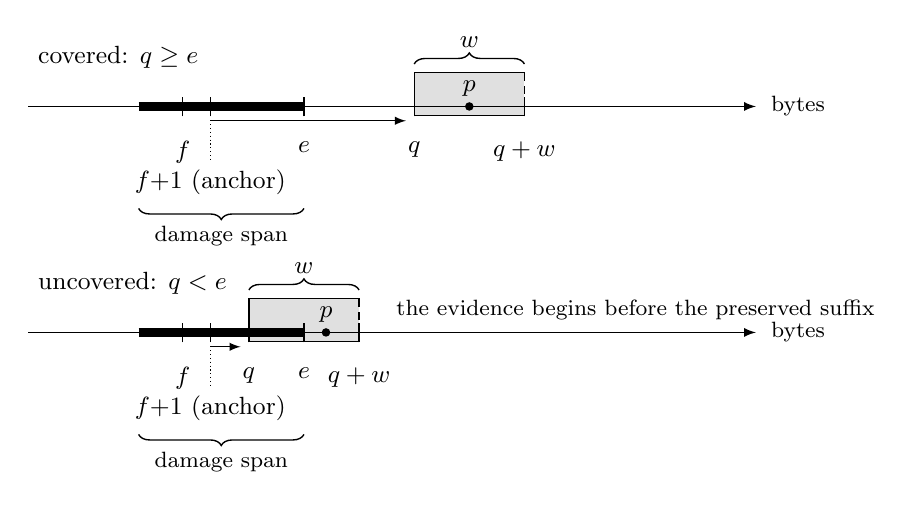
\begin{tikzpicture}[
    scale=0.70,
    x=1cm, y=1cm,
    axisline/.style={draw=black, line width=0.5pt, -latex},
    tick/.style={draw=black, line width=0.5pt},
    damage/.style={draw=black, line width=3pt},
    boxline/.style={draw=black, line width=0.5pt},
    lead/.style={draw=black, line width=0.4pt, densely dotted},
    brace/.style={draw=black, line width=0.5pt, decorate,
                  decoration={brace, amplitude=4pt, raise=1pt}},
    bracem/.style={draw=black, line width=0.5pt, decorate,
                   decoration={brace, mirror, amplitude=4pt, raise=1pt}},
    scan/.style={draw=black, line width=0.4pt, -latex},
  ]
  \begin{scope}[yshift=0cm]
    \fill[black!12] (7.0,-0.16) rectangle (9.0,0.62);
    \draw[axisline] (0,0) -- (13.2,0);
    \node[anchor=west, font=\footnotesize] at (13.3,0) {bytes};
    \draw[damage] (2.0,0) -- (5.0,0);
    \draw[boxline] (9.0,-0.16) -- (7.0,-0.16) -- (7.0,0.62) -- (9.0,0.62);
    \draw[boxline, densely dashed] (9.0,0.62) -- (9.0,-0.16);
    \foreach \x in {2.8, 3.3, 5.0, 7.0, 9.0} { \draw[tick] (\x,-0.18) -- (\x,0.18); }
    \fill[black] (8.0,0) circle (2.2pt);
    \node[anchor=south, font=\small, inner sep=2pt] at (8.0,0.08) {$p$};
    \draw[brace] (7.0,0.72) -- (9.0,0.72);
    \node[anchor=south, font=\small] at (8.0,0.89) {$w$};
    \draw[scan] (3.3,-0.26) -- (6.85,-0.26);
    \node[anchor=north, font=\small] at (2.8,-0.46) {$f$};
    \node[anchor=north, font=\small] at (5.0,-0.46) {$e$};
    \node[anchor=north, font=\small] at (7.0,-0.46) {$q$};
    \node[anchor=north, font=\small] at (9.0,-0.46) {$q+w$};
    \draw[lead] (3.3,-0.32) -- (3.3,-0.98);
    \node[anchor=north, font=\small] at (3.3,-0.98) {$f{+}1$ (anchor)};
    \draw[bracem] (2.0,-1.80) -- (5.0,-1.80);
    \node[anchor=north, font=\footnotesize] at (3.5,-2.00) {damage span};
    \node[anchor=west, font=\small] at (0,0.89) {covered: $q \geq e$};
  \end{scope}
  \begin{scope}[yshift=-4.1cm]
    \fill[black!12] (4.0,-0.16) rectangle (6.0,0.62);
    \draw[axisline] (0,0) -- (13.2,0);
    \node[anchor=west, font=\footnotesize] at (13.3,0) {bytes};
    \draw[damage] (2.0,0) -- (5.0,0);
    \draw[boxline] (6.0,-0.16) -- (4.0,-0.16) -- (4.0,0.62) -- (6.0,0.62);
    \draw[boxline, densely dashed] (6.0,0.62) -- (6.0,-0.16);
    \foreach \x in {2.8, 3.3, 4.0, 5.0, 6.0} { \draw[tick] (\x,-0.18) -- (\x,0.18); }
    \fill[black] (5.4,0) circle (2.2pt);
    \node[anchor=south, font=\small, inner sep=2pt] at (5.4,0.08) {$p$};
    \draw[brace] (4.0,0.72) -- (6.0,0.72);
    \node[anchor=south, font=\small] at (5.0,0.89) {$w$};
    \draw[scan] (3.3,-0.26) -- (3.85,-0.26);
    \node[anchor=north, font=\small] at (2.8,-0.46) {$f$};
    \node[anchor=north, font=\small] at (4.0,-0.46) {$q$};
    \node[anchor=north, font=\small] at (5.0,-0.46) {$e$};
    \node[anchor=north, font=\small] at (6.0,-0.46) {$q+w$};
    \draw[lead] (3.3,-0.32) -- (3.3,-0.98);
    \node[anchor=north, font=\small] at (3.3,-0.98) {$f{+}1$ (anchor)};
    \draw[bracem] (2.0,-1.80) -- (5.0,-1.80);
    \node[anchor=north, font=\footnotesize] at (3.5,-2.00) {damage span};
    \node[anchor=west, font=\small] at (0,0.89) {uncovered: $q < e$};
    \node[anchor=west, font=\footnotesize] at (6.5,0.40)
      {the evidence begins before the preserved suffix};
  \end{scope}
\end{tikzpicture}
\caption{The coverage split on one byte axis: failure offset $f$, blind anchor $f{+}1$, corruption end $e$, evidence
$[q, q{+}w)$ with the answer $p$ inside it. Above, covered evidence begins at or past $e$ and
Proposition~\ref{prop:oracle} applies at anchor $e$; below, uncovered evidence begins before the corruption end, the
anchor's $e \le q$ premise is unmet, and only the walk's guarantee at the blind anchor remains. The drawing is
schematic, not to scale, and its overlap with the damage span is one uncovered geometry, not the definition: uncovered
means only $q < e$.}
\label{fig:interval}
\end{figure}

\begin{table}[p]
\centering
\small
\setlength{\tabcolsep}{5pt}
\renewcommand{\arraystretch}{1.15}
\begin{tabular}{lrrrr}
\toprule
Row & Answers & Covered & Uncovered & Uncovered landed \\
\midrule
C-like, conventional & $7{,}356$ & $6{,}995$ & $361$ & $119$ \\
C-like, block comments & $4{,}754$ & $4{,}753$ & $1$ & $1$ \\
JSON, generated & $8{,}888$ & $8{,}051$ & $837$ & $554$ \\
C-like, split-friendly & $7{,}306$ & $6{,}817$ & $489$ & $291$ \\
C-like, bare & $7{,}877$ & $4{,}387$ & $3{,}490$ & $376$ \\
JSON, real document & $7{,}555$ & $7{,}138$ & $417$ & $248$ \\
\midrule
Total & $43{,}736$ & $38{,}141$ & $5{,}595$ & $1{,}589$ \\
\bottomrule
\end{tabular}
\renewcommand{\arraystretch}{1.0}
\caption{Evidence coverage per row, certified first answers only. Covered answers, evidence at or past the corruption
end, pass the asserted landing check, every one; uncovered answers sit outside the transfer premise, and their landings
are reported, never asserted.}
\label{tab:coverage}
\end{table}


\begin{table}[tbp]
\centering
\small
\setlength{\tabcolsep}{5pt}
\renewcommand{\arraystretch}{1.15}
\begin{tabular}{lrrrrrr}
\toprule
Row & Answers & Refusals & Landing & Overshoot & Attempts & Conv. \\
\midrule
C-like, conventional & $7{,}356$ & $0$ & $96.7\%$ & $25.3$ & $1.02$ & $28$ \\
C-like, block comments & $4{,}754$ & $0$ & $100.0\%$ & $164.9$ & $1.00$ & $169$ \\
JSON, generated & $8{,}888$ & $0$ & $96.8\%$ & $4.2$ & $1.03$ & $7$ \\
C-like, split-friendly & $7{,}306$ & $0$ & $97.3\%$ & $24.3$ & $1.02$ & $27$ \\
C-like, bare & $7{,}877$ & $0$ & $60.5\%$ & $4.3$ & $1.47$ & $3$ \\
JSON, real document & $7{,}555$ & $0$ & $97.8\%$ & $3.3$ & $1.02$ & $26$ \\
\bottomrule
\end{tabular}
\renewcommand{\arraystretch}{1.0}
\caption{Certified recovery pooled per row over the whole campaign: answers and refusals,
first-answer landing rate, mean absolute overshoot in bytes, mean recovery attempts per
incident, and mean signed convergence distance in bytes from the corruption end to where the
resumed boundary stream agrees with the mapped pristine one forever after. The bare row's
$60.5\%$ is its pooled landing rate. The block-comment
row's $164.9$ bytes accompanies the certificate sparsity the text discusses, and its convergence
decomposes into the same distance once rather than accumulating over attempts. Every figure recomputes from the archived
CSV through the checked-in analysis programs.}
\label{tab:pooled}
\end{table}


\FloatBarrier
\paragraph{Three patterns, each with the theorem's fingerprint.}
First, the pristine-repair transfer is assertable exactly where its evidence-preservation condition holds: the harness
checked every evidence-covered answer against its mapped pristine boundary, first answers and every later move alike,
and all $40{,}885$ move-level checks passed, the $38{,}141$ first-answer checks among them (Table~\ref{tab:coverage}
splits the coverage per row). Overall, certified recovery landed $90.8$\% of its $43{,}736$ first answers, Wilson
interval $[90.6, 91.1]$, refusing nothing in this campaign, and the pooled figure's entire distance from the
window-dense rows' $96.7$--$100$\% is one row's trusted-anchor price, taken up below. The classical conventions carry no
assertion clause anywhere: skip-one lands $10.0$\% pooled at $10.9$ recovery attempts per incident against the other
answering arms' $1.0$--$1.1$ (the semicolon variants average below one, their frequent first-move refusals contributing
zero attempts), and it alone exhausts the attempt budget, $776$ incidents. Second, where certificates are dense the
guarantee is also near: on the generated JSON row certified recovery's mean absolute overshoot is $4.2$ bytes against
newline-past's roughly thirty, and its resumed stream agrees with the mapped pristine one within a median of $6$ bytes
past the corruption. Third, where certificates are scarce the guarantee is honest about its price: on the block-comment
row the certified answers land $100$\% but $165$ bytes out on mean absolute overshoot, while newline-past lands $92.5$\%
at a fraction of the distance; the certificate promises soundness at its own position, never proximity, and on these
rows the price tracks certificate sparsity, an observed association rather than a measured law. One pooled number
belongs in plain sight rather than a footnote: the fresh-restart token-filtered newline convention lands $97.1$\%
pooled, above certified recovery's $90.8$\%, most of the pooled gap sitting in the bare row, whose price the coverage
split above stratifies; what it lacks is a repair-universal boundary guarantee behind any of those landings, a convergence more than twice as far (median $26$ bytes to certified recovery's $10$), and an answer at all where its delimiter
never occurs as a designated token, the refusal column the semicolon variants show at scale.

\paragraph{Short evidence is exposed: the byte path under damage.}
The bare C-like row, where every operator and punctuation byte certifies exactly, exercises the byte path at
scale. It also lands
worst, $60.5$\%
overall, Wilson interval $[59.4, 61.5]$, and the covered split decomposes that rate, within the one row and campaign
schedule, grouped by the returned certificate's kind, an observed stratification rather than a controlled
contrast: of the row's $2{,}408$
byte-evidence answers, $2{,}213$ rest on evidence not wholly in the preserved suffix, $91.9$ percent, and
none of them land, while of its $5{,}469$ window answers $1{,}277$ are uncovered, $23.3$ percent, and
$376$ land. All $4{,}387$ evidence-covered answers of the row pass the asserted landing check every time.
The within-row contrast is an observed association, not a randomized comparison, but it no longer leans on
the cross-row one, where evidence length is confounded with grammar and corpus; one reading consistent
with it is that a single byte is far easier for damage to produce than a two-to-four-byte occurrence with
the right context.

\paragraph{The mechanism behind coverage, from the archive.}
Coverage has a proved part and an observed part: the identity is proved algebraically, and the archive
recomputes the observed bins while checking every archived row against it.

\begin{lemma}[The overhang law]
\label{lem:overhang}
Call $h = e - f$ the damage's \emph{overhang} and $\ell = q - (f{+}1)$ the walk's \emph{evidence travel} for
that answer, the distance from the blind anchor to where the answer's evidence begins.
The answer is covered, $q \ge e$, exactly when $\ell \ge h - 1$; the search starts at the blind anchor,
so $\ell \ge 0$, and an overhang of at most one forces coverage.
\end{lemma}

\begin{proof}
$q \ge e$ rearranges to $q - (f{+}1) \ge (e - f) - 1$, and the walk's documented floor puts $q$ at or
past $f{+}1$.
\end{proof}

The threshold is sharp. For every $h \ge 2$ choose $n$ with $2n \ge h + 2$, and in $x = (\code{ab})^n$ replace
$\window{x}{2}{2+h}$ by the length-$h$ prefix of $(\code{ba})^\omega$. The corruption end is the one the operation
designates, $e = 2 + h$, exactly as everywhere else in this paper; this block is chosen because it also differs from $x$
at every replaced position, so the damage is actual across the whole designated span rather than merely designated, and
the instance stands under either reading of where the damage ends, the designated end and the byte-difference end, one past the last differing byte, alike.
Every \code{a} of a completely tokenizable string over $\{\code{ab}\}$ begins a token, so \code{a} is a certified byte.
The scan commits the leading \code{ab} and fails at $f = 2$; the blind search from three returns the certified \code{a}
at $q = p = 3$, and $q < e$ for every $h \ge 2$. So at every overhang at least two there is an uncovered certified
instance, and the lemma's threshold cannot be weakened.

\FloatBarrier
\begin{figure}[!htb]
\centering
\begin{tikzpicture}
\begin{axis}[
  ybar=0pt, bar width=4pt, width=\textwidth, height=5cm, area legend,
  ymin=0, ymax=105, ylabel={pooled landing rate (\%)},
  symbolic x coords={conventional, block, JSON, split-friendly, bare, real JSON},
  xtick=data, x tick label style={font=\small},
  legend style={at={(0.5,-0.18)}, anchor=north, legend columns=2, font=\small,
    /tikz/every even column/.append style={column sep=12pt}},
  ymajorgrids, tick label style={font=\small},
]
\addplot[fill=blue!65!black!80, draw=blue!65!black] table[col sep=comma, x=grammar, y=certified] {data/r6/r6-landing-figure.dat};
\addplot[fill=teal!70!black, draw=teal!50!black] table[col sep=comma, x=grammar, y=exact] {data/r6/r6-landing-figure.dat};
\addplot[fill=orange!80, draw=orange!60!black] table[col sep=comma, x=grammar, y=skip-one] {data/r6/r6-landing-figure.dat};
\addplot[fill=gray!45, draw=gray!70] table[col sep=comma, x=grammar, y=newline] {data/r6/r6-landing-figure.dat};
\addplot[fill=black!80, draw=black] table[col sep=comma, x=grammar, y=newline-at] {data/r6/r6-landing-figure.dat};
\addplot[fill=violet!60, draw=violet!80!black] table[col sep=comma, x=grammar, y=token-newline] {data/r6/r6-landing-figure.dat};
\legend{certified, exact, skip-one, newline-past, newline-at, token-newline}
% The two near-zero bars render as absent at this scale; their values are printed at the bars' own
% shifted positions so a missing series cannot be read where a collapse is the finding.
\node[font=\tiny, anchor=south, xshift=6pt] at (axis cs:bare,1) {$0$};
\node[font=\tiny, anchor=south, xshift=2pt] at (axis cs:real JSON,4) {$0.01$};
\end{axis}
\end{tikzpicture}
\caption{Pooled first-answer landing rate per row and arm, recomputed from the archived campaign. The raw
placements still flip between near-perfect and near-zero across rows; token filtering removed that failure
mode in this campaign, landing $97.0\%$ on the real document where its raw counterpart fails. Certified recovery needs no
placement convention, its one low row the trusted-anchor precondition; blind exact wins that row and loses
the conventional one, the complementarity the text takes up. The semicolon arms are in
Table~\ref{tab:quality}.}
\label{fig:landing}
\end{figure}

\begin{figure}[!htb]
\centering
\begin{tikzpicture}
\begin{axis}[
  width=0.85\textwidth, height=4.0cm,
  ymin=0, ymax=105, ylabel={rate (\%)},
  xlabel={overhang $e-f$, binned},
  xtick={1,2,3,4,5,6,7,8},
  xticklabels={$\le 0$, $1$, $2$, $3$, $4$--$7$, $8$--$15$, $16$--$31$, $32+$},
  tick label style={font=\small}, label style={font=\small},
  legend style={font=\small, at={(0.98,0.05)}, anchor=south east},
  ymajorgrids,
]
\addplot[mark=*, mark size=1.6pt, draw=black] table[x=bin, y=covered] {data/r6/r6-overhang.dat};
\addplot[mark=square*, mark size=1.5pt, draw=black!50, mark options={fill=black!12}]
  table[x=bin, y=landed] {data/r6/r6-overhang.dat};
\legend{covered, landed}
\end{axis}
\end{tikzpicture}
\caption{Coverage and first-answer landing for certified recovery against the damage's overhang past the
failure offset, recomputed from the archived CSV. Bin populations, left to right: $3{,}335$, $8{,}980$,
$1{,}133$, $2{,}733$, $9{,}708$, $5{,}103$, $11{,}558$, and $1{,}186$ answers. At overhang at most one the
anchor itself shelters the evidence and coverage is forced; every uncovered answer lives to the right.}
\label{fig:overhang}
\end{figure}

\paragraph{The known-clean arms.} The first half of that interface is measured rather than argued: an
oracle-aided campaign arm runs the same walk given the operation-designated start of the guaranteed-untouched
suffix, starting at the corruption end or
one past the failure, whichever is later, and a second oracle arm runs the exact decider from the same floor.
Their soundness arguments differ and both are asserted per trial: the clean walk's evidence is covered by
construction and every answer lands under the pristine transfer, while the clean decider returns no evidence and
its landings rest on complete-repair invariance with the pristine corpus the complete repair; $43{,}736$ first
answers each, the same count as the blind walk's, every one landing, with no refusals. The clean and blind walks
answer the same trials but not at the same places: their first positions differ on $4{,}592$ of the $43{,}736$
paired answers, $10.5$ percent, so what the truth about the damage changes is both which theorems cover the
answers and where a tenth of them land, the deployment precondition's content now a measured column rather than
advice.

\FloatBarrier
\paragraph{The real document.}
The ecological row runs the same JSON grammar over twitter.json, real Twitter API output. Certified recovery
does not notice the difference: $97.8$\% of its $7{,}555$ first answers land, mean absolute overshoot $3.3$ bytes.
The newline baselines expose the placement sensitivity the campaign measures as
outcome-critical,
which is why both placements are named. Newline-past collapses to one
landing in $7{,}555$ first answers, $0.01$\%: the document is pretty-printed, almost every newline is followed by
indentation, and skipping past the newline lands inside the run. Retained,
newline-at lands $96.9$\% here, by hitting the whitespace run the newline itself begins. Neither number
transfers: on the generated rows the same one-byte change runs the other way, pooled per row,
$98.0$\% falling to $26.6$\% on the conventional row, $92.5$\% to $1.3$\% on block comments,
$97.7$\% to $0.0$\% on bare,
where the
generated layout makes the newline mid-run and the byte after it a token start. The token-filtered form ends the
placement question the honest way: token-newline lands $97.0$\% on this document and $93.7$--$98.0$\% on
every generated row, because it never resumes inside a token its own scan just emitted, so the
token-filtered baseline both repairs the classical convention and removes its one-byte trap. Two
placements' worth of landing swing was a byte-level artifact; what no delimiter reading escapes is
availability and the missing repair-universal boundary guarantee. A raw delimiter convention's
landing rate is a layout property that a one-byte placement change swings between near-zero and near-perfect
in either direction; the certificate's soundness is placement-free and, for a fixed
automaton with preserved evidence, layout-independent, while availability, coverage,
refusal, and proximity remain corpus and layout properties, measured above, which is the
separation this row actually demonstrates.

\paragraph{Refusal is explicit and scoped.}
Certified recovery refused nowhere in this campaign, $43{,}736$ first answers on $43{,}736$ broken scans; its
refusal mode is real, pinned by fixture, and unexercised on these corpora under the rejection sampler. On the
window-dense rows every answer is a window answer, those grammars carrying no useful byte certificates; the
bare and split-friendly rows supply the byte path above, $2{,}408$ and $51$ byte-evidence answers. The
delimiter arms show what refusal looks like without a theorem: the semicolon variants each refuse over
fifteen thousand of the campaign's $43{,}736$ trials at the first move, over sixteen thousand terminally
once incidents that answered and then starved are counted, raw and token-filtered alike and nearly all on the
two JSON rows; the token-filtered form returns nothing at all on the real document, an observed result of this corpus:
its single pristine semicolon lies inside a string token that every restarted scan here happened to emit
whole, while the raw form's few answers
follow that in-string byte and land $0.7$ percent. Skip-one never refuses and lands rarely, $10.0$\% pooled,
the opposite failure.

\paragraph{The vacuity fence, stratified and then fenced again.} Every trial carries the verdict of the shipped
\code{minimal\_repair}, the routine's reported answer to whether any repair completes the blind tail: $26{,}928$
routine-labeled repairable against $16{,}808$ routine-labeled beyond repair, and the walk answered every one of the
latter, $38.4$ percent of its first answers. Assumption~\ref{ass:labels}, the label premise, is the one unproved input
this stratum consumes, and every claim resting on it below names it. Under the label premise the complete-repair reading
of Corollary~\ref{cor:complete} leaves those answers claiming nothing at the blind anchor, the vacuity question that
reading forces, and for $13{,}522$ of them the strengthened semantics is proved to fare no better: its quantifier
coincides with the complete-repair one without that assumption, so under the same premise it is empty exactly where that
one is; the rest stay undetermined in content, as follows. Every certified answer's evidence lies at or after its blind
search anchor, so Proposition~\ref{prop:collapse} needs only one further premise per trial, a one-attempt completed
resumed scan, and $13{,}522$ of the $16{,}808$ supply it: the $12{,}023$ whose evidence the damage spared and $1{,}499$
more on evidence not wholly in the preserved suffix. At all $13{,}522$ blind anchors the two quantifiers therefore
coincide, and under the label premise both are empty. Coincidence is in fact established far more widely, and without
invoking Assumption~\ref{ass:labels}: on the $26{,}928$ trials the routine labels repairable, every returned repair was
witness-verified by scanning, so $\Rcomp$ is inhabited by exhibition and Corollary~\ref{cor:dichotomy} forces the two
sets equal there independently of Assumption~\ref{ass:labels}. Equality therefore holds at $40{,}450$ of the campaign's
$43{,}736$ answers, $92.5$ percent, and only the $3{,}286$ remain candidates for strict inclusion at all; what the label
premise buys is not the equality but the reading of the equal sets as empty. The remaining $3{,}286$, whose first
resumed scans failed downstream, are the only answers this campaign leaves undetermined in content at the blind anchor
under the label premise: their soundness stands, and whether $\Rreach$ is inhabited there does not. Coverage never
entered that argument; what coverage decides is the transfer: the $12{,}023$ covered answers all landed, guaranteed at
the corruption-end anchor where the pristine corpus is a complete repair, the same guarantee the known-clean arms
exercise by construction, while the $1{,}499$ uncovered collapses carry no such transfer and land $1{,}066$ times as a
measurement, not a theorem. For uncovered evidence the corruption-end anchor is not a weaker fallback but no anchor at
all, the evidence beginning before it, outside the definition's domain, though each such answer stays governed by the
walk's soundness theorem at its own blind anchor. The deployment reading is the honest one: every returned answer is
sound at its blind anchor, and coverage decides which answers additionally carry Proposition~\ref{prop:oracle}'s
pristine transfer, the $12{,}023$ against the $1{,}499$. The failure offset cannot draw that line; the returned evidence
interval can, which is exactly why the evidence-returning form of the interface returns it.

\paragraph{The anchored decider, a different-property comparator.} The second machine in the campaign is the
library's anchored decider, whose documented contract is exactness for complete-repair invariance on
non-nullable sets: with the tail's end known to be the end of input, it answers the positions every completely
tokenizable repair agrees on and refuses tails no repair completes. That is a different predicate from the
certificates' evidence-reaching soundness, and the two separate on a two-token example: over $\{\code{ab},
\code{ba}\}$ the decider answers position zero of the tail \code{ab}, yet relative to the one-byte evidence
$\window{y}{0}{1}$ the repair \code{b} commits \code{ba} and dies having reached that evidence's image, with no
committed boundary at the answer's image, so the decider's answer is not evidence-reaching-invariant for that
interval. With the whole tail as evidence, reaching and completing already coincide, which is the decider's own
reading. The comparison below is therefore between two guarantees, not two implementations of one. The campaign
binds them where their properties overlap, and this revision tests both directions on the decider's direct call
at the blind anchor itself, its answer an archived column, never the advancing procedure: the direct call
answered every one of the $26{,}928$ routine-labeled-repairable trials at or before the walk, never once later,
which is not a coincidence of these rows:

\begin{proposition}[The decider never answers later than the walk]
\label{prop:order}
Fix a non-nullable token set and an anchor $c$. Suppose the walk, searching from $c$, answers $p$ on
evidence $\window{x}{q}{q+w}$ with $c \le q$, and the anchored decider, consulted at the same anchor
under its documented contract, which reports the earliest position at or after $c$ meeting its
certificate predicate, answers $d$. Then $d \le p$.
\end{proposition}

\begin{proof}
Every completely tokenizable repair is evidence-reaching, so by the resynchronization theorems a committed
token begins at $p$'s image in every complete repair anchored at $c$: the position $p$ is one the complete
repairs agree on. The decider's contract reports the earliest position at or after $c$ meeting that predicate, so
where it answers at all its answer $d$ is at or before every such position; $p$ is such a position,
hence $d \le p$. Exactness alone would not suffice: an invariant position that is not the earliest
could exceed the walk, so it is the contract's minimality, matched by the shipped
\code{next\_anchored\_start}, that the bound rests on.
\end{proof}

The measured containment is that proposition instantiated, worth $10{,}738$ bytes across
those trials, and on every routine-labeled-unrepairable trial it refused, a consistency regression between the
two routines rather than an independent proof, since both walk the same scenario machinery and their exactness
is a documented contract this paper assumes, its proof in a separate unposted draft and in neither posted
companion; every repair the routine did return was witness-verified by
scanning it against its tail. Run as a procedure, the decider answers everything and lands $89.8$ percent pooled
against the walk's $90.8$, and the per-row split is the finding: it wins the bare row, $89.1$ against $60.5$
percent, and loses the conventional row, $54.3$ against $96.7$, where an advanced anchor still sits inside a
broken string and anchored reasoning binds repairs of a damaged prefix, while the walk's occurrence-universal
certificates land wherever their evidence survived. Under the oracle floor both land on every trial, $100$
percent asserted, each under its own result: the clean walk under the pristine transfer, its evidence covered by
construction, and the clean decider under complete-repair invariance with the pristine corpus the complete
repair, the documented contract Table~\ref{tab:ladder} lists among the assumed inputs. The two machines are
complementary because their properties are: anchored completeness paid at this campaign's trustworthy anchors
and evidence-order search at its poisoned ones, two row-level contrasts rather than an anchor-class law, and at
$13{,}522$ of the poisoned anchors the surviving answers carry no evidence-reaching content either under the
label premise, only the clean-anchor transfer where their evidence is covered.

\paragraph{Convergence: what each convention costs the stream.} First landings decide where an arm resumes; convergence
measures what the choice costs downstream, the signed distance from the corruption end to where the resumed boundary
stream agrees with the mapped pristine one forever after, over completed incidents, with the boundaries from the
corruption end to that point counted lost, the initial jump included. The metric redistributes the credit twice over.
Skip-one, worst at landing, is the stream's best friend: it converges at median $2$ bytes and loses only $0.90$
boundaries per error pooled, at the price of $10.9$ attempts per incident, $0.9$ spurious starts per error inside the
divergence region, and $776$ budget exhaustions. Certified recovery converges at median $10$ bytes pooled, $2$ on the
bare row and $6$ on generated JSON, medians where the quality table's convergence column reports means, and loses $6.85$
boundaries per error pooled, from $0.22$ on the bare row to $34.6$ on block comments. On the block-comment row, where
every completed certified incident converges at its first answer, the lost boundaries are the initial jump the overshoot
already stated, the same quantity counted in tokens rather than bytes, appearing once rather than accumulating; on the
other rows a later move can lose boundaries the first answer did not skip. The newline conventions lose slightly more,
$8.01$ past and $7.42$ retained, at median $24$--$26$ bytes, and the semicolon forms lose a statement's worth, $24.4$,
$23.4$, and $24.5$ for past, retained, and token-filtered, at median about $60$, regardless of placement: the flip that
swings first landings between $0.01$ and $96.9$ percent on the real document moves convergence by roughly a token, so
the classical convention's real cost is the discarded remainder of the line, not the placement folklore. The
token-filtered semicolon form shows the availability cliff in stream terms: on the real document it refuses every
incident outright, its single candidate delimiter living inside a string token it now declines to treat as a
synchronizer.

\paragraph{The price of evidence order, measured.} The walk answers with the first certificate in evidence
order, not the smallest answerable position, and the campaign priced that fence: $90$ of the campaign's
$43{,}736$ certified first answers were nonminimal, by $90$ bytes in total, one byte each. The fence is real and
its cost on these rows is negligible, which is worth knowing before anyone complicates the walk to remove it.

\paragraph{Independent bounded verification.} A from-scratch maximal-munch reference model, written in Python
against only the public API and kept in the munch test suite as the recovery cross-check, is cross-checked
against the shipped library's own scan on $7.6$ million strings with zero disagreements, and drives bounded
exhaustive sweeps
over $89$ small non-nullable literal-token sets, boundaries and committed lengths the compared quantities, each
obligation carrying its own denominator. Walk soundness: $46{,}035{,}590$ (answer, repair) pairs, the
evidence-reaching premise holding on $1{,}308{,}265$ of them, no violations. The collapse proposition:
$836{,}387$ walk answers, its premise holding on $148{,}920$, no violations. The anchored decider:
$4{,}712{,}940$ (answer, completing repair) pairs, no violations, and never later than the walk on the
$174{,}368$ tails where the bounded search exhibits a completing repair and both answered. The routine's
negative labels: $95{,}836$, none refuted by any repair up to length four, the bounded reading of
Assumption~\ref{ass:labels}. Pristine transfer: an independently mapped damage sweep of $2.36$ million trials,
all $1{,}068{,}953$ covered answers landing, Proposition~\ref{prop:oracle} replicated without the harness. Every
quantifier is bounded where the contracts are not, and literal tokens leave regex structure and priority ties
outside the tested universe, so these runs are evidence, never proof; the drivers' executed negative controls
make a silent check an exit-failing defect of the cross-check itself; it runs in the munch test suite, where the
library it checks is built.

\begin{table}[bp]
\centering
\footnotesize
\setlength{\tabcolsep}{2.8pt}
\renewcommand{\arraystretch}{0.88}
\makeatletter
\begin{tabular}{llrrrrrr}
\toprule
Row & Arm & Answers & Landing & Overshoot & Conv. & Completed & Refused \\
\midrule
\@@input data/r6/r6-pooled-table.tex
\bottomrule
\end{tabular}
\makeatother
\caption{\small Every non-oracle arm pooled per row, three seeds of five hundred trials per cell, the body
generated by the archived analysis program and taken up verbatim. Columns: first-answer count and landing
rate, mean absolute overshoot, mean signed convergence distance, completed share, and terminal refusals,
incidents that never answered or answered and then starved, defined with the metrics above. The two oracle
arms are omitted as constant, $100$ percent landing on every row, asserted per trial; the per-cell grid over
three operations, three damage sizes, and three seeds is in the archived CSV, where the past placements
appear under their historic names newline and semicolon. Elsewhere the rows shorten, in this order, to
conventional (strings and line comments), block, generated JSON, split-friendly, bare, and real JSON. One
rounding is load-bearing: the real document's newline-past cell prints $0.0$ from exactly one landing in
$7{,}555$; the bare newline-at cell is a true zero.}
\label{tab:quality}
\end{table}


\enlargethispage{2\baselineskip}
\paragraph{Limitations and external validity.} Collected in one place: the corpora are generated except one
real-world document, the damage model is synthetic throughout, and real edit traces were not studied; cell sizes
are broken-scan counts and vary with absorption, and pooled rates carry Wilson intervals while individual cells
remain small in the absorbed strata; the third revision's schedule generator emitted fifteen-bit values, its
positions on a multiplicatively spread lattice of $32{,}768$ offsets per cell, disclosed in that archive's
record, and this revision replaces it with unbiased rejection sampling over the full span, three independent
seeds with every row's schedule and payload streams seeded apart, per-seed figures printed beside the pooled
ones and $43$ within-cell repeated draws counted; every arm now runs to a terminal outcome under one driver, so
the completed-incident view is a reported column rather than a gap, with a budget of one hundred attempts that
only skip-one ever exhausts; the anchored procedure's per-move cost, one scenario play per automaton state over
the remaining tail with jump-table construction that can reach quadratic in the tail and an advancing procedure
cubic in the worst case, was not priced against the walk's single forward scan, the comparison here being
quality alone; every campaign automaton is non-nullable, so the decider's nullable refusal is never exercised
and the comparison never leaves its domain; six rows over five grammars were measured, and none of the quality
figures generalize beyond them, since proximity, refusal, and exposure rates varied with certificate
density and evidence length, an association this campaign observed but did not isolate; the repairability labels
and the decider's refusals rest on the anchored routines' documented contracts, which this paper assumes and does
not prove, their proofs in a separate unposted draft and in neither posted companion, and the two routines share
their scenario machinery, so their agreement is consistency,
not independent confirmation. The byte path is exercised at scale by one grammar row, with $51$ further byte
answers on the split-friendly row. The search is the shipped form, whose window component searches lengths two
through four (the byte search is not length-capped), and the cap's sensitivity was not varied; the seam oracle
is conservative and applied uniformly, no claim is made that every sound position is discoverable by the
searched certificates, and throughput was deliberately not measured. The convergence metric compares whole
boundary streams, dropped tokens included, so it credits agreement rather than non-triviality; the lost and
spurious columns carry the divergence region's content. One grammar tried for the byte path refused to
participate at all: a log-line lexer, whose tokens are a run of non-newline bytes and the newline itself,
tokenizes every byte string, so no corruption can break its scan and recovery never fires.

\FloatBarrier

\section{Related work}


Panic mode is the textbook's simplest strategy at both levels: at the lexical level, delete successive
characters until a well-formed token appears, and at the parsing level, discard symbols until one of a
designated set of synchronizing tokens is found, usually delimiters such as semicolon, selected by the compiler
designer~\citep[pp.~88, 164--165]{dragon1986}. The guarantee attached is termination and, where a
synchronizer is found, membership in the designated set; what is not attached is any repair-universal
boundary guarantee for the position landed on, and the text itself notes that lexical panic-mode recovery
may confuse the parser. Our progress lemma reproduces the termination half of that classical guarantee,
membership following from the search rule where a delimiter convention is in force, and the
certificates add what it lacked, a theorem about the position landed on that ranges over repairs.

A close ancestor at the lexical level is Boullier and Jourdan's two-level scheme, which repairs table-driven
scanners and LR parsers alike: correction models specify insertions, deletions, and replacements around the
detection point, validated by the analyser accepting the model's trailing symbols, and when local repair fails
the parser skips to a grammar-writer key terminal while the scanner deletes the offending
character~\citep{boullier1987repair}. The classical comparator ideas have close antecedents here: the scanner's
deletion at the offending character is the nearest one-character antecedent of the skip-one convention, which
advances from the committed failure offset instead; the key-terminal skip anteceded the token-aware
designated-token discipline without supplying a repair-universal boundary guarantee; and the bounded correction
models carry a per-correction success test, continued acceptance. The scheme is the classical position at its
most parameterized: it chooses repairs and fallback recoveries judged excellent, mean, or poor against what a
human reader would have corrected, and it states operational acceptance conditions but no repair-universal
boundary property of the resume position. Repair invariance adds the missing quantifier for a scoped form of
exactly this design: once an anchor and its evidence are fixed, every prefix-local correction that preserves the
evidence and whose scan commits through it agrees at the certified position.

The repair school selects one concrete fix and validates it forward. Burke and Fisher~\citep{burke1987repair}
defer parse actions so repairs can be tried left of the error token, generate single-token candidates at each
trial point, and judge every candidate by the distance it lets the parse advance before blocking; a candidate
must advance at least one token in their implementation to remain in consideration, the farthest-checking
candidates are kept, and the pruning criteria were arrived at largely through experimentation with erroneous
Pascal and Ada programs; when simple recovery fails, scope closers are tried at the same trial points under
their own acceptance rules. Success means the correction a knowledgeable human reader would choose, a notion the
paper itself calls impossible to define precisely. The validation criterion concerns the proposed repair's
parse-ahead, never the position scanning resumes at, and nothing quantifies over the repairs not chosen, which
is exactly the quantification repair invariance makes.

Nearest in spirit is Richter's noncorrecting recovery: no correction is attempted, and the remainder of
the text is analyzed against the subword language, which buys provable properties about the error
messages, no spurious reports and no skipped text, with no assumptions about the nature of the
errors~\citep{richter1985noncorrecting}. Two of its 1985 observations anticipate this paper's
measurements: that panic mode trusts a single fiducial symbol ``to tell the parser where it is'' even
when ``a string of more than one symbol were less ambiguous'', which is the byte-versus-window distinction
the evaluation prices, and that the properties worth having are the provable ones. The deliverable still
differs the same way: subword membership says the damaged remainder can extend to a sentence, which is
repairability at the language level; repair invariance says where every such extension places a boundary.

The minimum-distance school fixes the metric rather than the position. Aho and Peterson~\citep{aho1972minimum} parse any
input to completion with the fewest possible errors, through a covering grammar whose error productions mark the
positions and kinds of the corrections, in time cubic in the input; they offer the algorithm as the yardstick for
evaluating recovery methods, and the textbook echoes exactly that framing while pricing it out of practice. The
quantification is the dual of ours: minimum distance searches over all repairs to return a minimum-error repair and its
parse, while repair invariance asks what every repair reaching the certificate's evidence agrees on, trading the richer
deliverable for the stronger quantifier. The school's modern member returns the whole optimum: Diekmann and Tratt's
CPCT+ reports the complete set of minimum-cost repair sequences at an error location, repairs $98.4$\% of $200{,}000$
real syntactically invalid Java programs within a half-second timeout each, and uses that completeness to report fewer
than half the error locations panic mode does on the same corpus~\citep{diekmann2020dontpanic}. The deliverable is
richer still, every best repair rather than one; the quantification is unchanged, over repairs to select among, never
over repairs to agree.

Incremental lexing maintains consistency across edits rather than certifying a recovery point across
hypothetical repairs. Wagner and Graham's general incremental lexer restarts the batch machine from saved states
at startable token boundaries and reproduces a batch scan of the incorporated text; errors are handled
representationally, by unmatched-text tokens and by error patterns recognizing near misses, and their
history-based alternative leaves invalid modifications unincorporated and retries them
later~\citep{wagner-lexing}. Hugo and Hansson's divide-and-conquer generator stores lexical errors in its
intermediate results, and the thesis also describes a local-error variant that lexes the following text from the
starting state~\citep{hugo2015incremental}. These works target batch or sequential agreement for the text they
incorporate; none states that a chosen position is a committed boundary in every repair of an unrepaired prefix
whose scan commits through the stated evidence.

Coding theory offers a longstanding form of the resynchronization question. A synchronizing word for a prefix
code drives the decoder into a known state from every state on which it is defined, so a complete decoder
realigns at each intact occurrence in the stream an error leaves behind, and a partial one, under the cited
definition, exactly where the word is defined from the state the error left. Almost all complete, equivalently
maximal, finite binary prefix codes admit such words as the number of codewords tends to
infinity~\citep{freiling2003sync}, and Ryzhikov and Szyku{\l}a study
the complexity of finding shortest ones, proving strong inapproximability for decoder-defined codes beside
algorithms for literal ones~\citep{ryzhikov2018sync}. Synchronizing words are the closest prefix-code analogue
of repair-independent reanchoring, and the certified byte is their lexical cousin. The general
setting does not transfer directly: maximal-munch token sets need not be prefix codes, one token may prefix
another, and commitment waits on lookahead and rollback, a decoder model the prefix-code results do not address;
the certificates quantify instead over repairs of the broken prefix, evidence-reaching failed scans included,
are decided statically per automaton, and refuse where their bounded search certifies nothing. The coding-theory
question is the existence and length of a universal resynchronizer for a code; ours is the soundness of one
position in one damaged input, under a scanning discipline whose rollback is exactly what desynchronizes the
decoder picture.

Three axes separate the lines above: what a position is keyed to, what its guarantee ranges over, and
what happens where nothing is found. Table~\ref{tab:axes} places the classical convention, the
lexical-level ancestor, the prefix-code analogue, and the certificates on those axes, each row argued
against its sources in the paragraphs above.


In deployment, tree-sitter aims, in its documentation's words, to be fast enough to parse on every keystroke and
robust enough to provide useful results in the presence of syntax errors, representing unrecognized text as
error nodes and inserted recovery tokens as zero-width missing nodes~\citep{treesitter}. The property claimed is
usefulness, stated operationally; no soundness property of the re-anchoring position is asserted, which is a
practical target the theorem here is meant to sharpen.

Where these lines single out a resume position at all, it is chosen by convention, validated by a score, or
inherited from history; to our knowledge, none states a property of a fixed broken-input position quantified
over every prefix repair whose scan commits through its supporting evidence, complete repairs the special case.
Repair invariance is exactly that scoped statement, and the certificates satisfying it were already posted for a
different purpose. Certified recovery does not prove that damaged input has a correct continuation; it
proves something narrower and operationally useful: whenever the search returns preserved evidence, every
repair whose scan commits through that evidence agrees on the returned boundary.

\begin{table}[!ht]
\centering
\small
\renewcommand{\arraystretch}{1.4}
\begin{tabular}{@{}>{\raggedright\arraybackslash}p{0.17\linewidth}p{0.22\linewidth}p{0.29\linewidth}p{0.24\linewidth}@{}}
\toprule
Line & Synchronizes on & Guarantee quantifies over & Failure or refusal \\
\midrule
Parser-level panic mode & designated synchronizing tokens, chosen by the designer, delimiters typically & nothing beyond
termination, and membership when a synchronizer is found; no repair-universal boundary guarantee &
no refusal; discards to a synchronizer or the input's end \\
\addlinespace[2.5pt]
Boullier and Jourdan & ordered correction models at the detection point; else key terminals & the chosen correction
only, by continued acceptance & local repair fails; key-terminal skip, character deleted \\
\addlinespace[2.5pt]
Synchronizing words for prefix codes & an intact occurrence of a synchronizing word & every decoder state
the word is defined on & partial decoders: possibly undefined from the error's state \\
\addlinespace[2.5pt]
This paper's certificates & a certified byte or certified window occurrence & every prefix repair whose
scan commits through the returned evidence & explicit refusal when no searched certificate lies ahead \\
\bottomrule
\end{tabular}
\renewcommand{\arraystretch}{1.0}
\caption{Three axes across the lines that re-anchor a damaged stream: what each line's search looks for in the input,
whom the resulting guarantee binds, and what happens when the search finds nothing. Each cell states only what its
paragraph argues from the sources: panic mode attaches termination and membership but no repair-universal boundary
guarantee, the two-level scheme's acceptance tests are per-correction, and synchronizing words speak about decoder
states rather than about repairs of a broken prefix. Panic mode, synchronizing words, and the certificates all search
the damaged input forward; the two-level scheme instead edits at the point of detection. The last row is the only one
whose guarantee ranges over repairs, complete repairs the special case, and the only forward search of the damaged input
here that refuses rather than consuming to the end.}
\label{tab:axes}
\end{table}

\FloatBarrier
\section{Conclusion}

Parser-level panic mode chooses a delimiter by convention; the certificates choose a resume position by theorem. A
position is a sound recovery point when every repair whose scan commits through the certificate's evidence places a
token boundary there, complete repairs the corollary; certified bytes and window origins supply such positions under the
stated anchor conditions; and the guarantee costs the committed-prefix lemma, a definition of reaching, and short proofs
on top of the companions' posted theorems. The procedure ships with its contract documented, its behavior pinned by
fail-closed tests, and the measurements say what the theorem buys: every evidence-covered answer passed its executable
landing check on every recovery move, $40{,}885$ of $40{,}885$; $90.8$\% of its first answers landed; the library's
anchored complete-repair decider, measured beside it as a different-property comparator, won the bare row and lost the
conventional one, both oracle-floored arms holding their contractual $100$ percent; the two repair readings are proved
equal at $40{,}450$ of the $43{,}736$ answers, $92.5$ percent, $26{,}928$ of them by a completing repair the harness
exhibited and scanned and $13{,}522$ by a resumed suffix that tokenizes whole, Assumption~\ref{ass:labels} needed only
to read the second group's coincident sets as empty, so only $3{,}286$ remain candidates for strict inclusion; and on the
generated JSON row,
where certificates are dense, newline-past's mean absolute overshoot is about seven times certified recovery's. Where
they are sparse it is honest about the price, and where the searched certificates end it refuses rather than guesses.
Claims end where the certificates do.

\Needspace*{8\baselineskip}
\section*{Tools}

Large language models were part of the workflow: drafting and revising the manuscript, verifying citations
against primary records, and reviewing the accompanying implementation. The author checked each
suggestion by direct derivation or against primary sources, the implementation, executable tests, and artifact
assertions, and is responsible for all content.

\begingroup
\setlength{\bibsep}{2pt}
\bibliographystyle{plainnat}
\bibliography{refs}
\endgroup

\end{document}
